%% RevTrace/FGCS manuscript skeleton (elsarticle, numbered references)
%% Decision: OUTLINE_V2_THEORY_GUIDED (docs/reports/revtrace_paper_outline_v2.md)
%% Claim discipline: no claim may exceed docs/CLAIM_BOUNDARIES.md.
%% Compile: pdflatex main && bibtex main && pdflatex main x2  (or Overleaf)
\documentclass[review]{elsarticle}

\usepackage{amsmath,amssymb,amsthm}
\usepackage{booktabs,multirow,array}
\usepackage{graphicx}
\usepackage{xcolor}
\usepackage{subcaption}
\usepackage{url}
\usepackage[hidelinks]{hyperref}

%% --- theorem environments (Section 3) ---------------------------------
\newtheorem{definition}{Definition}[section]
\newtheorem{theorem}{Theorem}[section]
\newtheorem{lemma}[theorem]{Lemma}
\newtheorem{corollary}[theorem]{Corollary}
\newtheorem{proposition}[theorem]{Proposition}
\newtheorem{assumption}[theorem]{Assumption}
\theoremstyle{remark}
\newtheorem{remark}[theorem]{Remark}

%% --- notation shortcuts (locked in outline v2, Section 1 ledger) ------
\newcommand{\state}{S}
\newcommand{\audio}{A}
\newcommand{\out}{Y}
\newcommand{\proj}{\Phi}
\newcommand{\ediv}{e}
\newcommand{\cont}{C}
\newcommand{\dist}{D}
\newcommand{\tx}{\tau}
\newcommand{\commit}{\Gamma}
\newcommand{\cert}{\mathrm{cert}}
\newcommand{\granratio}{\rho}

%% --- drafting aids (remove before submission) --------------------------
\newcommand{\todowrite}[1]{\textcolor{red}{[WRITE: #1]}}
\newcommand{\figplaceholder}[2]{%
  \fbox{\parbox[c][0.32\textheight][c]{\linewidth}{\centering\color{gray}FIGURE PLACEHOLDER --- #1}}%
  \caption{#2}}

%% --- table input path ---------------------------------------------------
\newcommand{\tbl}[1]{\input{tables/#1}}

\begin{document}

\begin{frontmatter}

\title{RevTrace: Dual-Granularity Feedback Transactions for
State-Certified Streaming ASR Serving}

%% Authors and affiliations: to be filled before submission.
\author{Author One\corref{cor1}}
\ead{author@example.org}
\cortext[cor1]{Corresponding author.}
\affiliation{organization={Affiliation}, country={Country}}

\begin{abstract}
%% Seven-sentence skeleton (outline v2). DRAFT v0 --- numbers are the
%% audited ones; wording will be polished in the final pass.
Streaming serving systems for revision-generative models treat generated
output as terminal, even when that output is written back into future model
state.
We formalize this class as revision-generative state machines and show that
batching-created output divergence becomes persistent state contamination
exactly when the feedback edge is present: with feedback, 8 of 21 legal
state pairs propagate divergence, and without it, none do.
We introduce Dual-Granularity Feedback Transactions (DGFT), which separate
low-latency display authority from coarse-grained state-write authority and
admit a revision to future state only as a certificate-bearing transaction;
same-granularity certification appears as the degenerate $\granratio=1$ case.
We prove three transaction invariants (uncertified-ancestry exclusion,
committed-state linearizability, granularity-independent safety) and derive
an authority-cost decomposition that predicts when coarse authority beats
same-granularity verification.
RevTrace, a runtime implementing DGFT with contract-scoped stratified
certification, is evaluated on two architecture families: Qwen3-ASR 0.6B/1.7B
and Whisper tiny/base/small.en, on two RTX 3090 GPUs.
On a shared bilingual workload, coarse-DGFT improves service throughput by
$1.39\times$ and $1.28\times$ over the same-granularity configuration while
the latter fails the 2\,s state-entry SLO at the session terminal; across
production contracts, DGFT reaches up to $6.88\times$ wall-clock speedup on
Qwen3-ASR-0.6B and passes all 16 Whisper serving cells, with zero
transaction-install violations in 320 Qwen revision events and 1{,}048
Whisper commits.
Risk signals schedule verification but never authorize state installation;
quality is measured against independent references per family and is never
pooled across contracts.
\end{abstract}

\begin{keyword}
streaming ASR serving \sep LLM inference \sep optimistic concurrency control
\sep state certification \sep transactional memory
\end{keyword}

\end{frontmatter}

%% =======================================================================
\section{Introduction}\label{sec:intro}
%% Section 1: Introduction. Jobs: field stake -> bottleneck -> prior
%% attempts -> what this paper does -> contributions. (outline v2 sec.3.1)

Streaming speech services are increasingly built on \emph{revision-generative}
models: a Whisper-style decoder is conditioned on its own previously generated
text~\cite{radford2023whisper,machacek2023whisperstreaming}, and ASR-capable
large language models such as Qwen3-ASR re-prompt themselves with rollback
prefixes of their prior output~\cite{shi2026qwen3asr}. In these systems the
generated text is not merely displayed; it is written back into the state that
conditions future generation. Serving systems, however, are still built on the
opposite assumption: a generated output is terminal, and its only consumer is
the user~\cite{kwon2023vllm,yu2022orca,zheng2024sglang}.

Batching is the standard mechanism by which serving systems buy throughput:
independent sessions share one forward pass~\cite{kwon2023vllm,agrawal2024sarathi,zhong2024distserve,sun2024llumnix}.
But batched execution perturbs floating-point arithmetic relative to singleton
execution, so batched outputs can differ locally from their canonical
single-session counterparts. In terminal-output systems this difference is
display noise. In revision-generative systems it is worse: once a perturbed
output is written into feedback state, the divergence is inherited by every
future revision. Section~\ref{sec:model} makes this precise; our causal
experiment confirms the prediction: with the feedback edge present, 8 of 21
legal state pairs propagate a batch-created divergence, and with the edge
removed, none do; on the persistent pairs the measured revision amplification
factor (RAF) reaches 153.

Prior mechanisms do not cover this failure mode. Streaming-ASR confirmation
policies such as LocalAgreement commit stable display prefixes but never
constrain which outputs may become future-state
parents~\cite{machacek2023whisperstreaming}. Speculative decoding verifies
draft tokens against a target distribution, not state-write
authority~\cite{leviathan2023specdec,chen2023specsample}. Deterministic-inference
work repairs arithmetic reproducibility but not feedback
semantics~\cite{xu2022deterministic,antunes2024reprohpc}. Optimistic
concurrency control supplies the closest analogy~\cite{kung1981occ,bernstein1983mvcc},
yet classical transactions commit reads and writes of stored data, whereas
here the ``write'' is a model-generated projection whose legality must be
certified by the serving contract itself.

This paper takes one position: \emph{revision outputs are speculative writes
to future model state, not merely user-visible responses}, and
\[
\mathrm{Display}(\out_t)\;\not\Rightarrow\;\mathrm{Authorize}\bigl(\proj(\out_t;\state_t)\bigr).
\]
We introduce \textbf{Dual-Granularity Feedback Transactions} (DGFT): a fine
proposal path serves low-latency display, while only a coarse canonical
authority may install state projections, and only as a certificate-bearing
transaction. DGFT is formalized in Section~\ref{sec:dgft}, where
same-granularity certification appears as the degenerate $\granratio=1$ case,
three transaction invariants are proved, and an authority-cost decomposition
predicts when coarse authority outperforms same-granularity verification.
\textbf{RevTrace} (Sections~\ref{sec:system}--\ref{sec:impl}) implements the
transaction runtime with a stratified, contract-scoped certification layer.

Contributions:
\begin{enumerate}
  \item A problem characterization of feedback-state contamination in
    revision-generative serving, with a causal verification that the feedback
    edge is the propagation channel (Section~\ref{sec:model},
    Section~\ref{sec:eval}, H1).
  \item DGFT, a dual-granularity transaction mechanism with provable
    invariants---uncertified-ancestry exclusion, committed-state
    linearizability, and granularity-independent safety---and a cost analysis
    whose predictions we test (Section~\ref{sec:dgft}, H3).
  \item RevTrace, a runtime with contract-scoped stratified certification:
    randomized audits and anytime-valid bounds on the same-granularity path,
    FP32 preflight invariance checks, exhaustive transaction validation, and
    independent quality references (Section~\ref{sec:system}, H2, H5).
  \item A cross-family evaluation on two architecture families and five
    checkpoints (Qwen3-ASR 0.6B/1.7B; Whisper tiny/base/small.en) on two
    RTX 3090 GPUs: same-workload SG/Coarse/Hybrid ablation, production
    performance, per-family quality contracts, and boundary evidence
    (Section~\ref{sec:eval}, H1--H5).
\end{enumerate}


\section{Model and Problem Formulation}\label{sec:model}
%% Section 2: Model and Problem Formulation. Owns all math objects.
%% Notation locked in outline v2 Section 1 ledger.

\begin{figure}[t]
  \centering
  \figplaceholder{F1 diptych (outline v2 sec.4): (a) ordinary batching ---
    audio revision, locally differing batched proposal displayed, output
    enters feedback state, trajectories diverge; corner annotation
    ``8/21 legal pairs propagate with feedback; 0/21 without; tail RAF up
    to 153 measured on the 6 persistent pairs''. (b) DGFT on the identical
    scenario --- local difference retained at display, state write denied,
    coarse authority later produces certificate, frontier advances.}
  {State-entry contamination under ordinary batching (a) and the same
  scenario under DGFT (b). DGFT does not require every provisional output
  to be identical; it prevents uncertified outputs from becoming
  future-state parents.}
  \label{fig:motivation}
\end{figure}

\subsection{Revision-generative state machines}\label{sec:model:rsm}

\begin{definition}[Revision-generative serving round]\label{def:rsm}
A serving round $t$ of a revision-generative system is a tuple
$(\state_t,\audio_t,\out_t)$ where $\state_t$ is the committed feedback
state entering the round, $\audio_t$ is the exogenous input (audio frontier),
and $\out_t$ is the generated output. The state update is
\begin{equation}\label{eq:state-update}
  \state_{t+1} = \mathcal{T}(\state_t,\audio_t,\out_t),
\end{equation}
where $\mathcal{T}$ is the model/adapter state-update function. The system is
\emph{revision-generative} when $\mathcal{T}$ depends on $\out_t$, i.e.\ the
output of round $t$ participates in the state read by round $t{+}1$.
\end{definition}

Not every byte of $\out_t$ enters future state. We isolate exactly the part
that does:

\begin{definition}[State projection]\label{def:projection}
The state projection $\proj(\out_t;\state_t)$ is the component of $\out_t$
that $\mathcal{T}$ consumes when forming $\state_{t+1}$. For Qwen3-ASR it is
the rollback prefix re-prompted at the next revision~\cite{shi2026qwen3asr};
for Whisper with previous-text conditioning it is the conditioning
prompt~\cite{radford2023whisper}.
\end{definition}

Ordinary batched serving makes an implicit assumption we name explicitly:
\begin{equation}\label{eq:implicit}
  \state_{t+1} = \proj(\out_t^{\mathrm{batch}};\state_t),
\end{equation}
i.e.\ whatever the batched forward pass produced may write state.
Equation~\eqref{eq:implicit} conflates ``was generated'' with ``may write
future state''.

\subsection{Display output versus state projection}\label{sec:model:display}

The user-facing display function may surface output that carries no
future-state authority: display-only suffixes, hold-back regions, and
provisional hypotheses are shown but excluded from
$\proj(\out_t;\state_t)$ by the adapter (Section~\ref{sec:system}). The
paper's central invariant separates the two permissions:
\begin{equation}\label{eq:invariant}
  \boxed{\;\mathrm{Display}(\out_t)\;\not\Rightarrow\;
  \mathrm{Authorize}\bigl(\proj(\out_t;\state_t)\bigr)\;}
\end{equation}

\subsection{State-entry divergence and contamination}\label{sec:model:divergence}

Let $\out_t^{f}$ be the fine (batched, proposer) output and $\out_t^{a}$ the
canonical authority output for the same round.

\begin{definition}[Local output divergence]\label{def:eps}
$\varepsilon_t = d_{\out}(\out_t^{f},\out_t^{a})$, with $d_{\out}$ an
output-space distance (mixed-unit edit distance in our contracts).
\end{definition}

\begin{definition}[State-entry divergence]\label{def:e}
$\ediv_t = d_{\state}\bigl(\proj(\out_t^{f};\state_t),\,
\proj(\out_t^{a};\state_t)\bigr)$, with $d_{\state}$ the state-space
distance induced by the same mixed-unit metric.
\end{definition}

\begin{definition}[Contamination event]\label{def:contamination}
Round $t$ is a contamination event $\cont_t$ iff the state projection of a
fine proposal is installed into committed state while $\ediv_t > 0$:
\[
  \cont_t \;:\Longleftrightarrow\; \ediv_t > 0 \;\wedge\;
  \proj(\out_t^{f};\state_t) \text{ installed into } \state_{t+1}.
\]
\end{definition}

Definition~\ref{def:contamination} upgrades the problem statement from
``outputs differ'' to ``a differing output acquired future-state write
permission''. Display-level instability literature observes the former;
this paper targets the latter.

\subsection{Feedback amplification}\label{sec:model:amplification}

Let $\dist_t = d_{\state}(\state_t^{f},\state_t^{a})$ be the trajectory
distance between the batched-served state trajectory and the canonical one.
A local perturbation decomposition gives
\begin{equation}\label{eq:recurrence}
  \dist_{t+1} \;\le\; L_t\,\dist_t \;+\; \beta_t\,\ediv_t ,
\end{equation}
where $L_t$ measures propagation of pre-existing difference and $\beta_t$
measures coupling of the round-$t$ state-entry divergence into the next
state. We make \emph{no} global Lipschitz claim: \eqref{eq:recurrence} is a
per-round decomposition with unknown coefficients, used only to identify
channels.

\begin{remark}[Causal prediction]\label{rem:causal}
Removing the feedback edge sets $\beta_t \equiv 0$, so a local state-entry
divergence can no longer enter $\dist_{t+1}$ through the revision channel.
Section~\ref{sec:eval} (H1) tests this prediction by intervention.
\end{remark}

\begin{definition}[Revision amplification factor]\label{def:raf}
For horizon $K$, the measured trajectory amplification factor is
\[
  \mathrm{RAF}_{t,K} \;=\; \frac{\dist_{t+K}}{\ediv_t + \epsilon_0},
\]
an empirical indicator of how one state-entry divergence propagates through
subsequent revisions. RAF is reported as a measured trajectory quantity, not
as a theoretical bound.
\end{definition}

\subsection{Design requirements derived from the model}\label{sec:model:reqs}

The model above forces four requirements on any serving mechanism that
claims to certify feedback state:
\begin{description}
  \item[R1 (Authority separation).] Display permission and state-write
    permission are distinct grants; Eq.~\eqref{eq:invariant}.
  \item[R2 (Parent ownership).] A state projection commits only onto the
    parent version it was computed against; otherwise staleness is
    undetectable.
  \item[R3 (Frontier monotonicity).] Committed audio frontiers advance
    monotonically---no gap, no overlap---so the committed history is a
    single sequence.
  \item[R4 (Evidence non-authority).] Statistical evidence (margins,
    coverage, repetition signals) schedules verification; it never
    authorizes installation.
\end{description}
R1--R4 reappear as protocol properties of DGFT
(Section~\ref{sec:dgft}), labels on the system diagram
(Figure~\ref{fig:arch}), and columns of the guarantee taxonomy
(Table~\ref{tab:guarantees}).


\section{DGFT: Theory and Mechanism}\label{sec:dgft}
%% Section 3: DGFT --- Theory and Mechanism. The theoretical core.
%% Theorem statements and proofs are drafted from the protocol invariants
%% actually enforced by the RevTrace runtime (exhaustive online validation:
%% 320 Qwen revision events + 1,048 Whisper commits, 0 violations).

\subsection{Transactions, certificates, and commits}\label{sec:dgft:tx}

DGFT wraps every state projection in a transaction. Throughout this section,
``committed state'' means the committed feedback sub-state $H$ of
Section~\ref{sec:model}; the remaining serving state $\state^{x}$ is never
written by generated output and therefore needs no certification.

\paragraph{Trust model.}
The authority coordinator and versioned ledger are trusted runtime
components; proposers and clients cannot mint or modify certificates. We
assume collision resistance of $h$, atomic certificate consumption with the
ledger compare-and-swap, and immutable session audio bytes once covered by a
certificate. The threat model excludes a Byzantine authority or compromised
ledger. A digest provides content binding, not standalone authentication;
authenticity follows from issuance inside the protected coordinator.

The protocol theorems do not assume a deterministic proposer, greedy
decoding, synchronous GPU kernels, or equality of proposer KV caches. The
authority may use greedy, beam, or sampled decoding provided that the realized
projection and the complete decoding/runtime configuration (including any
randomness policy needed by the contract) are bound by $\chi_j$. Asynchrony is
allowed because the parent-version compare-and-swap serializes installation.
The theorems certify provenance and installation legality, not semantic
correctness of the authority output or repeatability of an independently
rerun stochastic authority.

\begin{definition}[DGFT transaction]\label{def:tx}
A transaction is the object
\[
  \tx_t = \bigl(\mathrm{sid},\, e,\, p,\, v_{\mathrm{parent}},\,
  [a_s,a_e),\, \out_t,\, \proj(\out_t;H_t),\, \mathrm{cert}_t\bigr),
\]
comprising the session id, contract epoch $e$, policy $p$, the parent state
version read, the audio frontier interval covered, the generated output,
its state projection, and the certificate it carries (pending for fine
proposals, issued for authority commits). The proposal granularity
$g_p$ (fine window) and the authority granularity $g_a$ (coarse canonical
segment) define the granularity ratio $\granratio = g_a/g_p \ge 1$.
\end{definition}

\begin{definition}[Certificate]\label{def:cert}
An authority certificate is a binding record
\[
\begin{aligned}
  \cert_j = \mathrm{Bind}\bigl(&\mathrm{sid}_j,e_j,p_j,v_j,
  [f_j,f_{j+1}),\\[-2pt]
  &h(\audio_{[f_j,f_{j+1})}),h(\proj_j^{a}),\chi_j\bigr),
\end{aligned}
\]
where $\proj_j^{a} = \proj(\out_j^{a};H_{v_j})$ is the canonical state
projection computed by the authority against parent version $v_j$, and
$h(\cdot)$ is a content digest over immutable bytes. The configuration
digest $\chi_j$ binds the model checkpoint, tokenizer, decoding parameters,
projection adapter, numerical precision, and authority-runtime version. A
certificate therefore binds
exactly one canonical projection to exactly one commit tuple; it is issued
only when the contract's authority checks pass, and it is single-use:
consumed by the commit that presents it.
\end{definition}

\begin{definition}[Commit validity]\label{def:commit}
An authority commit is a tuple
\[
  \commit_j = (\mathrm{sid}_j,\, e_j,\, p_j,\, v_j,\, [f_j,f_{j+1}),\,
  \proj_j^{a},\, \cert_j).
\]
$\commit_j$ is \emph{valid}, written $\mathrm{Valid}(\commit_j)$, iff
(i) session, contract epoch, and policy match the live session fence;
(ii) $v_j$ equals the currently committed parent version;
(iii) $[f_j,f_{j+1})$ continues the committed frontier without gap or
overlap; and
(iv) certificate binding: $\cert_j$ binds exactly the presented fields, the
digest $h(\proj_j^{a})$ recomputes from the presented projection, and the
certificate has not been consumed before. Only valid commits mutate
committed state.
\end{definition}

Definitions~\ref{def:tx}--\ref{def:commit} realize requirements
R1--R4 (Section~\ref{sec:model:reqs}) structurally: display never produces
a commit (R1), $v_j$ enforced inside the certificate binding gives parent
ownership (R2), $[f_j,f_{j+1})$ enforces frontier monotonicity (R3), and
$\cert_j$ is issued only by authority checks, never by risk signals (R4).
Table~\ref{tab:guarantees} previews how these properties separate DGFT from
weaker protection regimes; the guarantee claims are evaluated in
Section~\ref{sec:eval} (H2, H5).

\tbl{t5_guarantees}

\begin{definition}[Committed provenance ancestry]\label{def:ancestry}
A projection $P$ is an ancestor of committed state $H_j$ iff $P$ labels an
accepted ledger transition on the unique path
$H_0\rightarrow H_1\rightarrow\cdots\rightarrow H_j$. Displayed proposals
and rejected transactions are not ancestors.
\end{definition}

\subsection{Theorem 1: uncertified-ancestry exclusion}\label{sec:dgft:thm1}

\begin{theorem}[Uncertified-Ancestry Exclusion]\label{thm:ancestry}
If committed state is updated exclusively through commits satisfying
$\mathrm{Valid}$ (Definition~\ref{def:commit}), then no fine projection
that is not bound by a valid certificate can become part of the ancestry of
any future committed state in the sense of Definition~\ref{def:ancestry}.
\end{theorem}

\begin{proof}
By induction over the commit sequence $\commit_1,\commit_2,\ldots$.
Base: the initial committed state $H_0$ is contract-defined, so its
ancestry contains no generated output. Step: assume committed state $H_j$
has ancestry containing only certificate-bound projections. The next state
$H_{j+1}$ arises only from a valid $\commit_{j+1}$; by
Definition~\ref{def:commit}(iv), commit application installs exactly the
projection whose digest is bound by $\cert_{j+1}$, since any other content
fails the binding check and is rejected. A fine projection
$\proj(\out^{f};H)$ that differs from the certified canonical projection
$\proj_{j+1}^{a}$ therefore cannot be installed by $\commit_{j+1}$; if a
fine proposal happens to coincide bitwise with $\proj_{j+1}^{a}$, what
enters state is the certified content, attributable to the authority's
certificate rather than to the uncertified fine generation. Provisional
display never mutates committed state by construction of the runtime
(Section~\ref{sec:system}), completing the induction.
\end{proof}

Theorem~\ref{thm:ancestry} is deliberately architecture-agnostic: it depends
on the commit protocol, not on margin accuracy, model determinism,
FP16/FP32 agreement, or the choice of ASR family.

\subsection{Theorem 2: fork-free committed-state linearity}\label{sec:dgft:thm2}

\begin{theorem}[Fork-Free Committed-State Linearity]\label{thm:linear}
Assume commit application is atomic: the validity checks of
Definition~\ref{def:commit} and the state installation execute as one
indivisible compare-and-swap against the committed state, and each
certificate is consumed by at most one commit. Then, under parent-version
checking (Definition~\ref{def:commit}(ii)) and frontier-continuity checking
(Definition~\ref{def:commit}(iii)), the accepted commits of a session form
a fork-free, gap-free, overlap-free linear history of feedback state.
\end{theorem}

\begin{proof}
Atomicity closes the check-then-act race: two distinct commits cannot both
observe the same committed state, both pass the checks, and both install.
Parent-version checking then makes the accepted commits a tree of height at
most one per version: two distinct commits cannot both satisfy
$v_j = \mathrm{version}(H)$ against the same committed state, so the
history is fork-free. Single-use consumption excludes replay of an
already-consumed certificate against a later parent. Frontier-continuity
checking orders accepted intervals $[f_j,f_{j+1})$ into a sequence with
$f_{j+1} = f'_{j}$ for consecutive commits, excluding gaps and overlaps.
Hence the accepted commits are a single linear sequence.
\end{proof}

\begin{remark}[Scope of the concurrency claim]\label{rem:not-linearizable}
Theorem~\ref{thm:linear} proves a serial accepted-commit history with the
ledger compare-and-swap as its serialization point. It is not a claim of
full Herlihy--Wing linearizability for every client invocation and response;
such a claim would require a separate concurrent-object history and
real-time-order specification~\cite{herlihy1990linearizability}.
\end{remark}

\begin{corollary}[Stale-descendant rejection]\label{cor:stale}
A revision computed against a stale parent, i.e.\
$v_{\mathrm{parent}} \neq \mathrm{version}(H_j)$, cannot legally commit.
It fails Definition~\ref{def:commit}(ii) and is rejected without mutating
state.
\end{corollary}

\subsection{Theorem 3: granularity-independent safety}\label{sec:dgft:thm3}

\begin{theorem}[Granularity-Independent Safety]\label{thm:gran}
For any granularity ratio $\granratio \ge 1$, if every authority segment
starts at the committed parent, covers a contiguous audio frontier, yields a
legal state projection, and passes the certificate and version checks of
Definition~\ref{def:commit}, then the conclusions of
Theorems~\ref{thm:ancestry} and~\ref{thm:linear} hold.
\end{theorem}

\begin{proof}
The proofs of Theorems~\ref{thm:ancestry} and~\ref{thm:linear} use only the
certificate binding of Definition~\ref{def:cert}, the validity predicate of
Definition~\ref{def:commit}, and atomic commit application; none of their
steps depends on the size of $[f_j,f_{j+1})$ relative to the fine window.
Varying $\granratio$ changes how much audio a single certificate covers,
not which commits are admissible.
\end{proof}

\begin{corollary}[Same-granularity certification as $\granratio=1$]\label{cor:sg}
Setting $\granratio = 1$ makes proposal and authority granularities
coincide: the directional coverage witness degenerates to the identity and
fine replay degenerates into risk-triggered re-verification. The
same-granularity (SG) configuration is therefore a reduction of DGFT under
the same protocol, not a separate mechanism.
\end{corollary}

\begin{remark}[Canonical-path boundary]\label{rem:canonical}
Corollary~\ref{cor:sg} identifies the protocol, not the arithmetic path: in
our contracts SG runs an FP16 singleton authority while Coarse/Hybrid run an
FP32 batched authority. These are distinct canonical paths; we claim
protocol equivalence, never bitwise identity.
\end{remark}

\subsection{Authority-cost decomposition}\label{sec:dgft:cost}

The safety results above are silent about cost; the following analysis is a
proposition with explicit assumptions, whose predictions we test
(Section~\ref{sec:eval}, H3). Let $B$ be the number of concurrent sessions,
$q$ the SG verification fraction, $r$ the Hybrid selective-replay fraction,
$C_s$ the singleton authority cost per covered region, $C_c(\granratio,B)$
the batched coarse authority cost per segment, $C_{\mathrm{commit}}$ the
transaction/commit overhead, and $Q_s$ the queueing/fragmentation cost of
singleton authority. Then
\begin{align}
  T_{\mathrm{SG}}^{a} &\approx q\,B\,\granratio\,C_s \;+\; Q_s, \label{eq:cost-sg}\\
  T_{\mathrm{DGFT}}^{a} &\approx C_c(\granratio,B) \;+\;
    r\,B\,\granratio\,C_s \;+\; C_{\mathrm{commit}}, \label{eq:cost-dgft}
\end{align}
and end-to-end service time is governed by the slower lane plus repair:
\begin{equation}\label{eq:cost-service}
  T_{\mathrm{service}} \approx \max(T_p, T^{a}) + T_{\mathrm{repair}},
\end{equation}
with proposer and authority running concurrently on separate GPUs.

\begin{proposition}[Model-based operating condition]\label{prop:coarse}
Let end-to-end service time be given by
Eq.~\eqref{eq:cost-service}. Coarse-DGFT improves service throughput over
SG whenever
\[
\begin{split}
  &\max\bigl(T_p,\; C_c(\granratio,B) + rB\granratio C_s +
  C_{\mathrm{commit}}\bigr) + T_{\mathrm{repair}}^{D} \\
  &\quad <\; \max\bigl(T_p,\; qB\granratio C_s + Q_s\bigr)
  + T_{\mathrm{repair}}^{S}.
\end{split}
\]
A simplified sufficient condition, applicable when the authority lane is on
or near the critical path in both configurations ($T^{a} \ge T_p$) and the
repair costs are comparable, is
\[
\begin{split}
  &C_c(\granratio,B) + rB\granratio C_s + C_{\mathrm{commit}} \\
  &\quad <\; qB\granratio C_s + Q_s .
\end{split}
\]
In particular, even a small verification fraction $q$ leaves SG paying
singleton invocation and queueing costs across all $B$ sessions, while a
batched coarse authority amortizes them into $C_c$.
\end{proposition}

Equations~\eqref{eq:cost-sg}--\eqref{eq:cost-dgft} motivate four empirical
hypotheses rather than determine them without fitted costs: (P1) a burst of
singleton authority work can create an SG tail even at 8--10\% verification;
(P2) a batched coarse authority can amortize invocation and queueing costs;
(P3) Hybrid may trade replay fraction $r$ for quality at a performance and
energy cost; and (P4) the ordering can reverse across models because the
complete authority paths---including precision and execution mode---have
model-dependent costs. Section~\ref{sec:eval} tests these hypotheses on the
same workload. Because SG and Coarse/Hybrid use different canonical
arithmetic paths in our implementation (Remark~\ref{rem:canonical}), the
comparison identifies integrated operating points, not a precision-independent
causal effect of $\granratio$ alone.

\subsection{Operating-point trade-offs}\label{sec:dgft:tradeoff}

A deployment selects SG, Coarse, or Hybrid as configuration policy $\pi$,
trading latency, energy, and quality subject to hard safety:
\[
  \max_{\pi}\ J(\pi)
  \quad\text{s.t.}\quad V(\pi)=0,\ C(\pi)\leq B,
\]
where $J$ aggregates the deployment objective, $V$ counts transaction
violations, and $C(\pi)\leq B$ denotes the contract's display and quality
caps.
DGFT supplies the safety-constrained operating envelope; the three evaluated
contracts instantiate three operating points. We do not solve this
optimization online and do not claim any single operating point dominates:
the measured ordering is workload- and model-dependent
(Section~\ref{sec:eval}, H3).


\section{The RevTrace System}\label{sec:system}
%% Section 4: The RevTrace System. Three-element pattern per module:
%% motivation / mechanism / evidence hook. (outline v2 sec.3.4)

RevTrace implements DGFT as a transaction runtime: per-family adapters, a
versioned ledger, and a stratified certification layer
(Figure~\ref{fig:arch}).

\begin{figure*}[t]
  \centering
  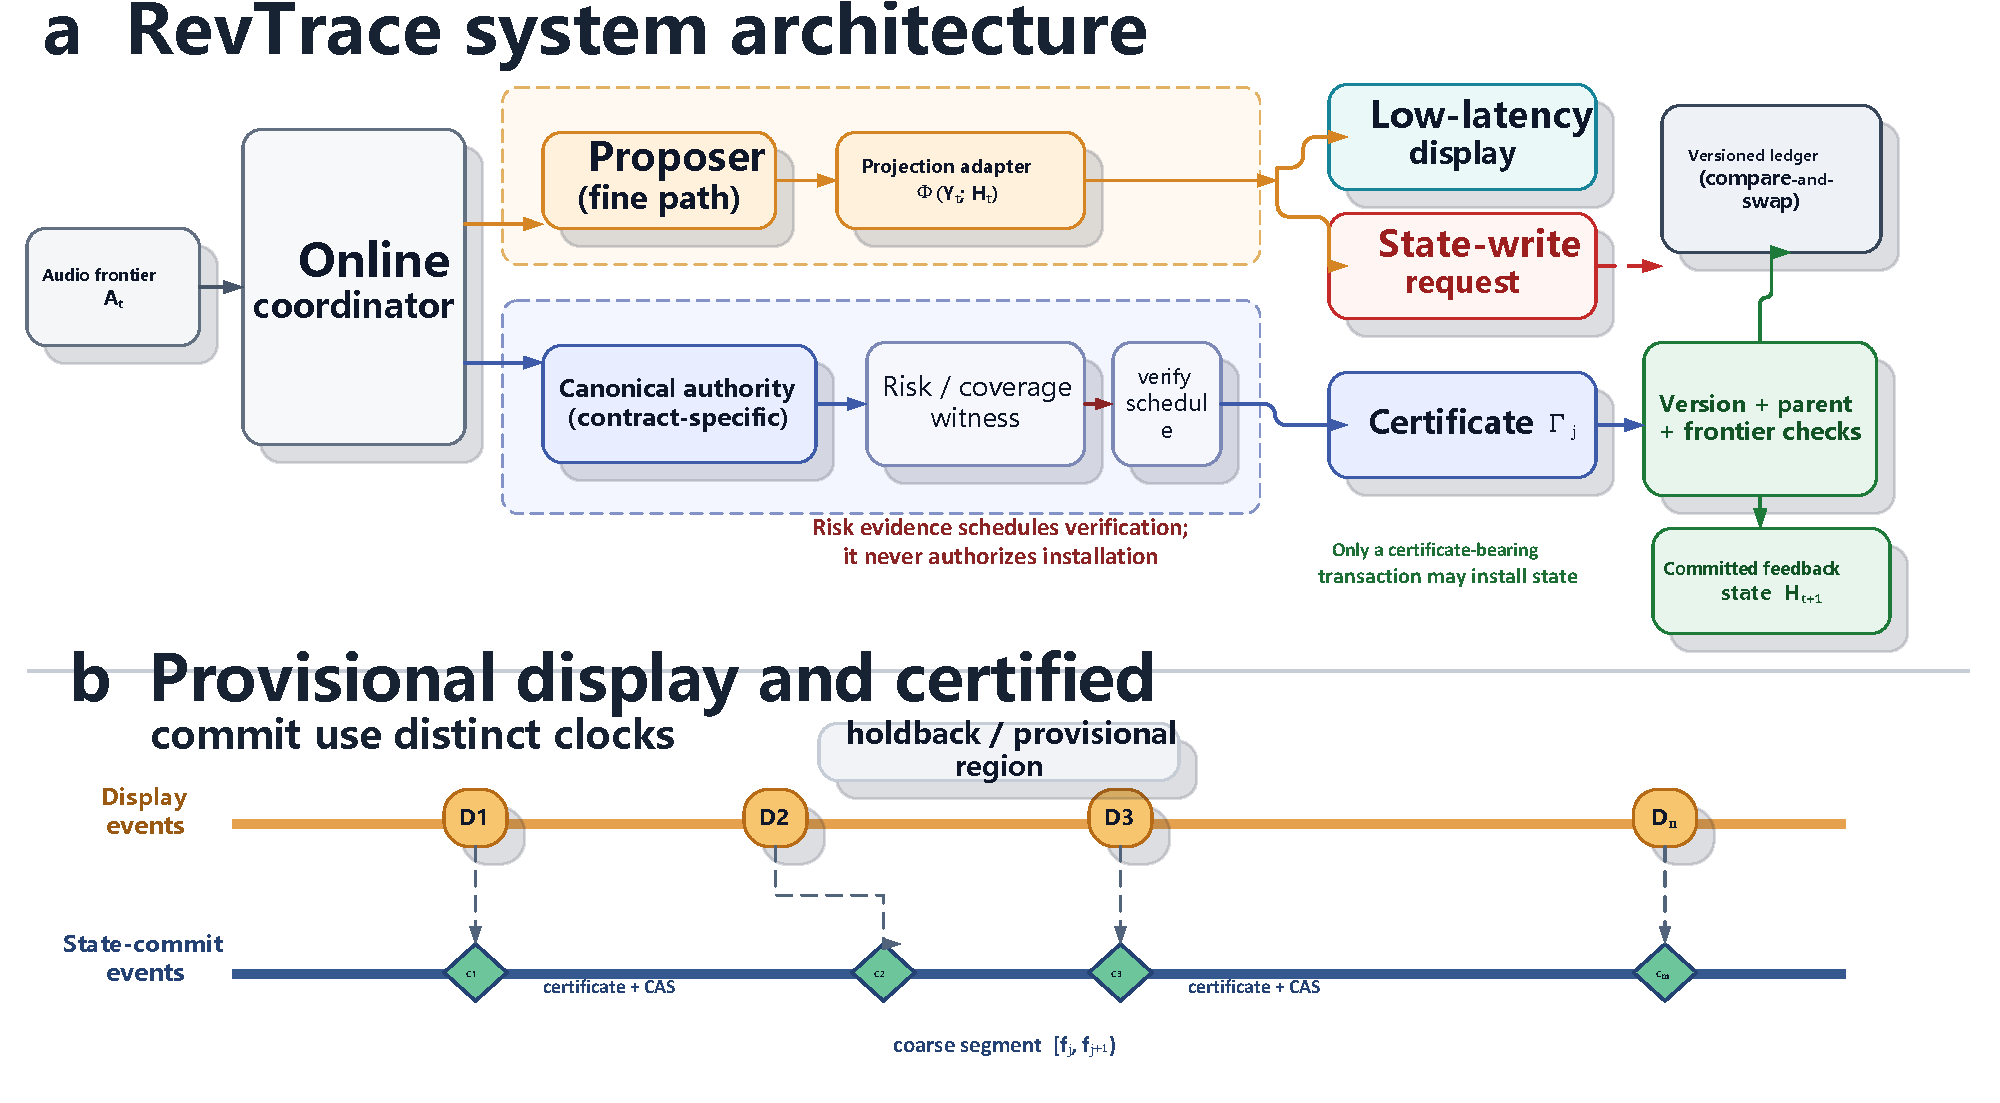
\includegraphics[width=\textwidth]{figures/f2_architecture_visio.pdf}
  \caption{RevTrace architecture (top) and the DGFT commit timeline (bottom).
  Provisional display and state write are separate permissions; only a
  certificate-bearing transaction whose parent version and frontier checks
  pass may advance committed state. Risk and coverage evidence may schedule
  verification but cannot authorize installation.}
  \label{fig:arch}
\end{figure*}

\subsection{Architecture-specific adapters}\label{sec:sys:adapters}

\emph{Motivation.} The safety proofs of Section~\ref{sec:dgft} require only
three interfaces; everything family-specific must stay out of the protocol.
\emph{Mechanism.} Each family provides (i) a state-projection adapter
computing $\proj(\out_t;H_t)$ (Qwen rollback prefix; Whisper
previous-text prompt), (ii) an authority adapter executing the canonical
path (FP16 singleton for SG; FP32 batched for Coarse/Hybrid), and
(iii) an evidence adapter collecting risk signals (margins, directional
coverage, repetition) for the certification layer.
\emph{Evidence hook.} H4 (Section~\ref{sec:eval}) runs the identical
runtime over both families through these adapters.

\subsection{Certificate and versioned ledger}\label{sec:sys:ledger}

\emph{Motivation.} R2/R3 require detecting staleness and frontier
discontinuity at commit time. \emph{Mechanism.} A compare-and-swap-style
ledger stores committed state versions; every commit tuple
$\commit_j$ (Definition~\ref{def:commit}) is checked against session,
contract epoch, policy, and state-version fences before installation, and
each accepted commit consumes its certificate exactly once.
\emph{Evidence hook.} H2: exhaustive transaction validation reports every
install attempt against these fences (320 Qwen events; 1{,}048 Whisper
commits; zero violations).

\subsection{Directional coverage and selective fine replay}\label{sec:sys:coverage}

\emph{Motivation.} A coarse authority segment must be witnessed against the
fine proposals it replaces; replaying everything would forfeit the point of
coarse authority. \emph{Mechanism.} The coverage witness records, in Latin
and CJK units, which fine-region outputs the coarse certificate accounts
for; uncovered regions are queued for fine replay. Hybrid adds
risk-triggered replay at fraction $r$, trading cost for quality
(Eq.~\eqref{eq:cost-dgft}). \emph{Evidence hook.} H3 ablates $r=0$
(Coarse) against $r>0$ (Hybrid) on the same workload.

\subsection{Stratified certification}\label{sec:sys:cert}

Four strata, each with a non-transferable scope
(Figure~\ref{fig:cert}):
(i) \emph{SG numerical risk}: randomized audits of the singleton authority
with anytime-valid (UCB) bounds, scoped to the SG adapter
path~\cite{howard2021confidence,ramdas2023savi};
(ii) \emph{authority implementation}: contract-scoped FP32 preflight
invariance checks (batch repeat, batch-vs-singleton), fail-closed;
(iii) \emph{transaction integrity}: exhaustive online validation of
certificates, versions, and frontier continuity;
(iv) \emph{semantic quality}: independent per-family references.
A risk signal from any stratum may schedule verification but never authorize
installation (R4).

\begin{figure}[t]
  \centering
  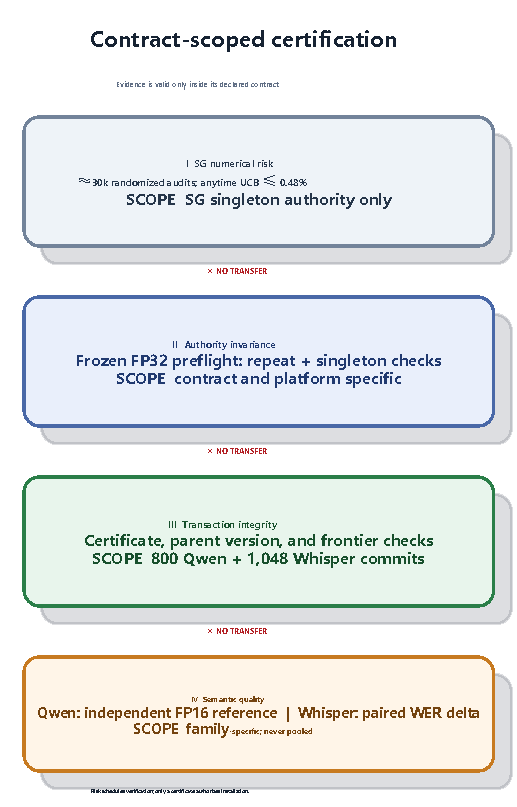
\includegraphics[width=\columnwidth]{figures/f3_certification_visio.pdf}
  \caption{Stratified, contract-scoped certification. Each rung yields exactly one
  scope-limited guarantee; no rung's evidence authorizes another's
  installation decisions.}
  \label{fig:cert}
\end{figure}

\subsection{Online coordinator}\label{sec:sys:coord}

The coordinator schedules the proposer and authority lanes on separate
GPUs (Eq.~\eqref{eq:cost-service}), invalidates stale descendants
(Corollary~\ref{cor:stale}), closes terminal frontiers at session end, and
performs rollback/rebase when a commit supersedes displayed provisional
state.


\section{Implementation}\label{sec:impl}
%% Section 5: Implementation. Keep short; cite artifacts.

RevTrace is implemented as a serving runtime for revision-generative ASR
models. The Qwen rollback adapter maintains a growing audio buffer with
prefix rollback and holdback semantics; the Whisper prompt adapter maintains
previous-text conditioning state~\cite{shi2026qwen3asr,radford2023whisper}.
The coarse authority executes in FP32 with a 4{,}096-token KV-cache bound
per session; the one-time contract preflight (batch-repeat and
batch-vs-singleton invariance) takes 10.7--11.1\,s and is excluded from
steady-state service timing, reported separately
(Section~\ref{sec:discussion}). Sessions arrive online and are scheduled
with causal arrival ordering; decoder outputs are transferred to the host
via vectorized paths. Experiments use two NVIDIA RTX 3090 GPUs, one
hosting the proposer lane and one the authority lane. Realizations rejected
during closure and measurement repairs are documented in
\ref{app:repairs}. All evaluated numbers are bound to code commit,
contract digest, and result hashes in the release. The source
code, frozen audited artifacts, and analysis scripts are publicly available
in the RevTrace repository
(\url{https://github.com/zhouz4884-coder/RevTrace}).

The independent scale-out contract uses one RHEL~7.6 node with eight
Tesla V100 PCIe GPUs (32\,GB each), PyTorch 2.4.1, CUDA 12.1, and the
Transformers-eager backend. It runs replicas rather than distributed model
parallelism: up to four proposal workers and four authority workers share a
versioned commit queue. Input audio is deterministically resampled to 16\,kHz.
This contract has its own environment fingerprint, raw cell records, worker
diagnostics, and result hashes; its absolute timing is never pooled with the
RTX~3090/vLLM contract.


\section{Evaluation}\label{sec:eval}
%% Section 6: Evaluation as five hypothesis tests. Each subsection:
%% theory prediction -> experiment -> numbers -> verdict.
%% Every number below is audited: results/r10_qwen_cross_adapter/
%% ablation_summary.json (G1); R10 cross-adapter report; R9.E closure
%% report and results/r9_dgft/FINAL_REPORT_ONLINE.json; Phase 4B causal
%% experiment. Scopes are stated with every number.

\subsection{Experimental setup and claim contracts}\label{sec:eval:setup}

Table~\ref{tab:contracts} fixes, per family and per model, the proposal
path, authority path, workload contract, quality reference, and the claims
each contract supports; no number is ever pooled across these contracts.
Hardware: two RTX 3090 GPUs. Workloads: the shared bilingual 30\,s
16-session contract (c16, 480\,s audio) for the same-workload ladder, and
the per-family production contracts for cross-architecture evidence.

\tbl{t1_claim_contract}

\subsection{H1: state divergence propagates through the feedback edge}
\label{sec:eval:h1}

\emph{Prediction} (Remark~\ref{rem:causal}): setting $\beta_t \equiv 0$ by
removing the feedback edge eliminates propagation of batch-created
state-entry divergence.
\emph{Experiment.} On the Whisper family we enumerated the 21 legal state
pairs and intervened causally: the identical perturbation was applied with
the feedback edge present and with it removed.
\emph{Result.} With feedback, 8 of 21 legal pairs propagate the divergence;
without feedback, 0 of 21. On the 6 persistent pairs the measured tail RAF
(Definition~\ref{def:raf}) reaches 153.
\emph{Verdict.} The prediction is confirmed: the feedback edge is the
propagation channel, and contamination is therefore a state-authority
problem, not a display problem.

\subsection{H2: transaction invariants exclude uncertified ancestry}
\label{sec:eval:h2}

\emph{Prediction} (Theorems~\ref{thm:ancestry}--\ref{thm:gran}): if the
runtime enforces Definition~\ref{def:commit}, no install violation,
fork, gap, or overlap occurs in any completed trace.
\emph{Experiment.} Exhaustive online validation of every transaction install
attempt: 320 Qwen revision events (R10 cross-adapter matrix, four cells) and
1{,}048 Whisper commits (R9.E, 16 cells), including stale-descendant
attempts and terminal frontier closure.
\emph{Result.} Zero transaction-install violations, zero output/state
violations, zero batch-repeat mismatches, zero batch-vs-singleton mismatches;
stale commits: 0 accepted (rejection exercised, Corollary~\ref{cor:stale});
all sessions closed with monotone terminal frontiers.
\emph{Verdict.} The invariants hold exhaustively on the evaluated traces.
We report this as exhaustive-trace protocol validation; it is not a
failure-probability-zero claim for unobserved workloads.

\subsection{H3: authority granularity drives performance}\label{sec:eval:h3}

\emph{Prediction} (Proposition~\ref{prop:coarse}, P1--P4): coarse authority
beats SG on throughput; SG shows terminal-burst tail failures even at
8--10\% verification; Hybrid pays for quality in performance and energy; the
energy ordering may reverse across models.

\begin{figure}[t]
  \centering
  \figplaceholder{F3 double panel (outline v2 sec.4): (a) Pareto scatter,
    x = wall speedup, y = P95 edit rate, size = service energy (J), color =
    SG/Coarse/Hybrid, markers for 0.6B and 1.7B; (b) latency-scope
    dumbbells --- SG state-entry P99 vs DGFT display P99 and segment-commit
    P99, axes labeled by latency semantics.}
  {Same-workload operating points (c16). Coarse-DGFT is the throughput
  point, Hybrid the quality-conservative point, and SG the same-granularity
  certification point; latency scopes are never mixed on one axis.}
  \label{fig:ablation}
\end{figure}
\emph{Experiment.} Same-workload ladder on the identical 16 bilingual 30\,s
sessions (c16): SG ($\granratio=1$, FP16 singleton authority, verification
fractions 8.3\%/9.6\%), Coarse-DGFT ($\granratio=3$, FP32 batched authority,
$r=0$), Hybrid-DGFT ($\granratio=3$, $r>0$), on Qwen3-ASR 0.6B and 1.7B.
\emph{Result} (Table~\ref{tab:ladder}, Figure~\ref{fig:ablation}).
Coarse-DGFT improves service throughput by $1.39\times$ (0.6B) and
$1.28\times$ (1.7B) over SG while cutting wall-clock service time by
27.8\% and 21.6\%. SG fails the 2\,s state-entry deadline at the session
terminal (miss rates 3.33\%/4.17\%; state-entry P99 2.735/2.964\,s) and is
SLO-failed, whereas Coarse/Hybrid pass with display P99
$\le 1.018$\,s. Hybrid holds throughput near SG ($1.03\times$ on 0.6B) at
lower edit rate (2.15\% vs 3.43\% P95) but costs energy
($+16.8\%$ vs SG on 0.6B; $+54.2\%$ on 1.7B, where Hybrid also loses
throughput, $0.85\times$). The direct energy comparison against SG reverses
between models: Coarse saves 4.4\% on 0.6B but consumes 15.1\% more on
1.7B.
\emph{Verdict.} Predictions P1--P4 are all confirmed, including the
model-dependent reversal of the energy ordering. The SG configuration
remains the same-granularity certification point (Corollary~\ref{cor:sg}),
not a dominated baseline.

\tbl{t2_ladder}

\subsection{H4: one invariant holds across adapters}\label{sec:eval:h4}

\emph{Prediction} (Section~\ref{sec:sys:adapters}): the protocol needs only
projection/authority/certificate interfaces, so one runtime serves
structurally different revision semantics.
\emph{Experiment and result.} On Qwen3-ASR (rollback, holdback, growing
buffer), the R10 production matrix reaches $6.88\times$ wall-clock and
$3.44\times$ GPU-normalized speedup with 59.8\% energy reduction
(0.6B, Coarse-DGFT), and $6.06\times/3.03\times$ with 51.0\% energy
reduction (1.7B), at P95 mixed-unit edit rates $\le 3.43\%$ against an
independent FP16 singleton reference and display P99 $\le 1.018$\,s. On
Whisper (previous-text conditioning), the identical runtime passes 16/16
production cells with median wall-clock speedup $2.841\times$
(2.633--3.849 across cells), $1.421\times$ GPU-normalized, 31.13\% energy
reduction, display P99 $\le 1.492$\,s, and 1{,}048 certificates with zero
violations.
\emph{Verdict.} Confirmed: the invariant transfers across two architecture
families through adapters; performance magnitudes are family- and
model-dependent and are reported per contract.

\begin{figure}[t]
  \centering
  \figplaceholder{F4 cross-architecture production matrix (outline v2
    sec.4): Qwen 4 operating points + Whisper 16 cells (per model/arrival
    group); wall-clock, GPU-normalized, and energy bars or panels.}
  {Cross-family production evidence under per-contract baselines.}
  \label{fig:production}
\end{figure}

\tbl{t3_production}

\subsection{H5: each certification layer guarantees only its scope}
\label{sec:eval:h5}

\emph{Prediction} (R4, Section~\ref{sec:sys:cert}): evidence strata are
non-transferable; each yields a bounded statement about its own scope.
\emph{Result, by stratum.}
(i) SG numerical risk: randomized audits of the SG authority path
($\approx$30k audits, checkpoints 20\,s/120\,s) give anytime-valid UCBs of
0.480\%/0.478\%; this bound belongs to the SG adapter path only and is not
transferred to DGFT paths~\cite{howard2021confidence}.
(ii) Authority implementation: the contract-scoped FP32 preflight records
zero batch-repeat and zero batch-vs-singleton mismatches on the frozen Qwen
contract (10.7--11.1\,s, excluded from service timing).
(iii) Transaction integrity: H2's exhaustive validation (0 violations on
320 events + 1{,}048 commits).
(iv) Semantic quality, per family and never pooled: Qwen mixed-unit edit
rate against the independent FP16 singleton reference has P95 $\le 3.43\%$
(worst 5.41\%, zero catastrophic cases; exact sessions rise from 11/16 to
13/16 on 0.6B Hybrid and from 9/16 to 10/16 on 1.7B); Whisper paired WER
deltas against unprotected feedback are all negative, $-12.23$/$-18.21$/$-25.27$
points on dev for tiny/base/small.en (bootstrap uppers
$-10.48$/$-16.17$/$-22.15$) and $-8.26$/$-11.03$/$-13.76$ on 214 untouched
utterances (uppers $-5.15$/$-7.51$/$-9.09$)
(Figure~\ref{fig:quality}).

\begin{figure}[t]
  \centering
  \figplaceholder{F5 double panel (outline v2 sec.4): (a) Qwen edit-rate
    CDF against the FP16 singleton reference with exact-session counts;
    (b) Whisper paired WER deltas (dev + untouched) with bootstrap upper
    bounds. Two estimands, two panels, no pooled axis.}
  {Per-family quality contracts. Qwen measures distance to an independent
  canonical reference; Whisper measures improvement over unprotected
  feedback.}
  \label{fig:quality}
\end{figure}
\emph{Verdict.} Each layer produces exactly one scope-limited guarantee;
no stratum's evidence is used to authorize another's installation
decisions.

\tbl{t4_quality}


\section{Discussion and Boundaries}\label{sec:discussion}
%% Section 7: Discussion and Boundaries. (outline v2 sec.3.7)

\paragraph{FP32 authority is a canonical path, not a repair.}
The FP32 batched authority defines a new canonical reference for the
contract; it is not a bitwise repair of FP16 arithmetic. FP16 remains the
proposer and SG-authority precision. Quality estimands are defined against
the FP16 singleton reference (Qwen) and against unprotected feedback
(Whisper); neither claims bitwise equivalence across precisions.

\paragraph{Risk evidence does not transfer.}
The SG-path UCB of 0.480\% bounds the numerical risk of the SG adapter's
randomized audits. It is never applied to Coarse/Hybrid paths, whose safety
rests on Theorems~\ref{thm:ancestry}--\ref{thm:gran} and exhaustive
transaction validation instead.

\paragraph{The authority plane is trusted and versioned.}
The current contract assumes a non-Byzantine authority coordinator, atomic
certificate consumption and version comparison, immutable audio bytes during
a transaction, and collision-resistant digests. A certificate binds the
parent version, audio and projection digests, and the complete canonical-path
configuration; it is not a standalone proof against a compromised authority.
Our production traces contain no stale-install attempt. Their zero observed
install violations therefore validate accepted-history integrity, whereas
the stale-result rejection rule is supported by the protocol argument rather
than a fault-injection denominator.

\paragraph{Quality estimands differ by family.}
Qwen edit rates measure distance to an independent canonical reference;
Whisper WER deltas measure improvement over unprotected feedback. The two
answer different questions and are never pooled into a single quality
number.

\paragraph{Virtual arrival versus wall clock.}
Production cells schedule virtual causal arrivals; service wall-clock and
energy meters measure real GPU work. Latency columns are labeled by
semantics (display, state-entry, or segment-commit) wherever they appear.
Consequently, the SG certified state-entry deadline and the DGFT provisional
display/segment-commit measurements are reported separately; the manuscript
does not transfer an SLO pass label between them.

\paragraph{Why coarse authority improves throughput.}
The same-workload ablation supports the cost decomposition rather than a
granularity-only explanation. SG repeatedly invokes an FP16 singleton
authority and accumulates a synchronized terminal burst; Coarse amortizes
authority work through an FP32 batch, while Hybrid pays selective replay to
recover a more conservative quality point. This explains why Coarse has the
shortest absolute wall time, why Hybrid is not uniformly dominant, and why the
ordering may change with model-specific FP16/FP32 cost. Unlike token-level
verified speculation such as LLM-42~\cite{zhang2026llm42}, the saved work here
is measured at a revision-state authorization boundary; unlike stateful cache
reuse~\cite{yu2025pensieve,gao2024cachedattention}, the protected object is the
transition that creates reusable state.

\paragraph{The cost equations are a decomposition, not a fitted oracle.}
Equations~\eqref{eq:cost-sg}--\eqref{eq:cost-service} identify the complete
authority-path terms and yield a sufficient operating condition; they do not
claim a workload-independent numerical predictor. H3 therefore compares
complete configurations on one frozen workload and reports the model-dependent
ordering reversal. Risk-bound sensitivity is evaluated separately and is
never converted into fabricated per-setting GPU times.

\paragraph{Preflight amortization.}
The one-time contract preflight costs 10.7--11.1\,s. With per-session
steady-state savings $\Delta T = T_{\mathrm{baseline}} - T_{\mathrm{DGFT}}$,
we define the break-even point as
$N = \lceil T_{\mathrm{preflight}} / \Delta T \rceil$ sessions. We report
the one-time cost and steady-state results separately, and exclude the
preflight from all service timing.

\paragraph{Not every ASR system needs DGFT.}
The original Voxtral report studies multimodal audio understanding and
long-context transcription~\cite{mistral2025voxtral}; Voxtral Realtime instead
uses a natively streaming delayed-stream design~\cite{mistral2026voxtralrealtime}.
Such append-only semantics expose no rollback-style feedback write path, so
the contamination channel of
Section~\ref{sec:model:amplification} is absent; at low concurrency (our c8
capacity probe) batching pressure is small. DGFT targets the
revision-generative operating regime where feedback writes and batching
coexist.

\paragraph{Scale boundary.}
Under the stated trust and atomicity assumptions, safety is independent of
adapter and granularity, but performance remains hardware- and
backend-specific. The RTX~3090 results establish cross-architecture mechanism
portability over five checkpoints. The independent 8$\times$V100 experiment
adds single-node replica scaling and identifies c64 as the largest measured
point satisfying the 2\,s display SLO; c128 saturates and fails that SLO.
Neither experiment establishes multi-node scalability or a data-center
production claim. The V100 result also shows that even FP32 batching need not
match singleton output, so its authority contract is platform-scoped rather
than assumed from precision alone. Higher-end accelerators and distributed
authority ledgers may change the cost ordering without changing the
state-write authorization problem.


\section{Related Work}\label{sec:related}
%% Section 8: Related Work. Collision-matrix framing; synthesize, do not
%% list. (outline v2 sec.3.8)

\paragraph{Streaming ASR and confirmation policies.}
Streaming decoders must decide when displayed text becomes final.
Whisper-based streaming maintains confirmed/unconfirmed prefixes and commits
a prefix only after repeated decoding passes agree
(LocalAgreement)~\cite{machacek2023whisperstreaming,radford2023whisper};
chunk-based adaptations add truncation
detection~\cite{wang2024simulwhisper}. These policies protect \emph{display}
stability; none of them constrains which outputs may become parents of
future model state, which is exactly the gap
Eq.~\eqref{eq:invariant} names.

\paragraph{Speculative execution with verification.}
Speculative decoding verifies draft tokens against a target model so that
acceleration preserves the output
distribution~\cite{leviathan2023specdec,chen2023specsample}. The analogy is
structural---propose fast, verify before accepting---but the verified object
differs: tokens of a single response, rather than a state projection that
conditions all future rounds.

\paragraph{LLM serving systems.}
Modern serving systems optimize memory, scheduling, and parallelism for
throughput and latency: paged KV-cache management~\cite{kwon2023vllm},
iteration-level scheduling~\cite{yu2022orca}, structured-program
runtimes~\cite{zheng2024sglang}, prefill-decode
chunking~\cite{agrawal2024sarathi}, phase
disaggregation~\cite{zhong2024distserve}, and dynamic request
migration~\cite{sun2024llumnix} (surveyed
in~\cite{miao2023servingsurvey}). All treat generated output as terminal:
none models the case where outputs are written back into the state that
conditions future generation. RevTrace is complementary to, not competitive
with, these efficiency mechanisms.

\paragraph{Determinism and reproducibility of inference.}
Training- and inference-time nondeterminism from nondeterministic kernels
and atomic accumulation is well
documented~\cite{xu2022deterministic,antunes2024reprohpc}. DGFT takes the
opposite position: instead of promising bitwise determinism of batched
execution, it treats batch-created divergence as given and governs which
divergent outputs may write future state.

\paragraph{Concurrency control.}
Optimistic concurrency control validates transactions at
commit~\cite{kung1981occ}; multiversion schemes track data
lineage~\cite{bernstein1983mvcc}. DGFT borrows the transactional
discipline---parent ownership, version fencing, linearizable commit
history---but the validated object is a model-generated state projection
whose legality is certified by the serving contract, not by stored-data
consistency alone.

\paragraph{Anytime-valid statistics.}
Confidence sequences and e-value-based testing provide evidence measures
valid under optional stopping~\cite{howard2021confidence,ramdas2023savi,
grunwald2024safetesting}. RevTrace uses them in exactly one stratum: to
bound the numerical risk of the SG adapter's randomized audits, with the
bound explicitly scoped to that path.

%% Pre-submission sweep: extend this section (or an appendix table) with
%% any streaming/stateful-serving work found to jointly handle
%% batch-created divergence + feedback propagation + state-entry authority.


\section{Conclusion}\label{sec:conclusion}
%% Section 9: Conclusion. (outline v2 sec.3.9)

Revision-generative serving turns generated outputs into speculative writes
to future model state. This paper formalized the resulting contamination
channel and introduced certificate-bearing transactions that separate
display authority from state-write authority. Under the stated trust and
binding assumptions, the protocol excludes uncertified ancestry, produces a
single fork-free committed revision history, and remains safe for any
granularity ratio. Its cost is governed by the complete authority path---not
granularity alone---and the measurements identify when coarse authority is
worthwhile. Across two architecture families and five checkpoints, RevTrace
reaches up to $6.88\times$ wall-clock speedup. We observe no output/state or
transaction-install violations in 800 Qwen revision events (480 SG and 320
DGFT) and 1{,}048 Whisper commits; these finite traces support the declared
contracts but are not a proof of zero implementation faults. Same-granularity
certification is the $\granratio=1$ reduction of the protocol. Risk signals
schedule verification but never authorize installation, and quality evidence
does not transfer across estimands or canonical paths.
On an independent single-node 8$\times$V100 contract, balanced
four-proposer/four-authority scaling sustains $147.1\times/114.5\times$ audio
real-time throughput for Qwen3-ASR 0.6B/1.7B at c64, with display P99
1.115/1.471\,s and nominal scale efficiency 91.1/100.7\%. The c128 points fail
the 2\,s SLO and are retained as the measured capacity boundary. These values
extend the evidence to high-concurrency single-node serving without being
pooled with the RTX~3090/vLLM contract.
Implementing the session-partitioned ledger across nodes and measuring its
consensus/commit cost, and extending the transaction discipline to other
feedback-driven text and multimodal revision models, are the natural next
steps.


%% =======================================================================
\bibliographystyle{elsarticle-num}
\bibliography{refs}

\end{document}
